\chapter{Visualization of geographical data.}


\pagestyle{fancy}

When working with a GIS, most of the time we will visualize the data we work with. Although certain data, such as satellite images or maps from a map server, include their own rendering and can be visualized \emph{as they are}, in most cases is the user of a GIS who defines the way geographical data is rendered. In other words, the GIS user \textbf{takes the role of the cartographer} and for this reason, must be familiar with the ideas and techniques used by cartographers.

Along with the concepts and tools from classic cartography, GIS include elements from what is known as \textbf{scientific visualization}, such as \textbf{interactivity} or \textbf{multidimensional data rendering}. This approach, richer than the classic one from cartography, is known as \textbf{geovisualization}.

In this chapter, we will see some fundamental ideas about data visualization, and how they are applied to both the traditional field of cartography and the GIS and geovisualization context.

\section{Basic ideas about data visualization}

When we visualize any kind of geographical information, whether on a computer screen or on a printed map, we are using a \textbf{visual language} to convey that information. 

The study of signs of a language is called \textbf{semiology}. In the case of a visual language, we have a \textbf{graphic semiology}. This semiology works with the signs of the language that we use to visualize geographical data and helps us understand why and how visual elements serve their purpose of correctly conveying the information from which they are created.

\subsection{Visual variables}

Visual elements have several properties that can be used to transmit information. Depending on the case, some of them might more suitable than others.


\begin{figure}[!hbt]
\centering
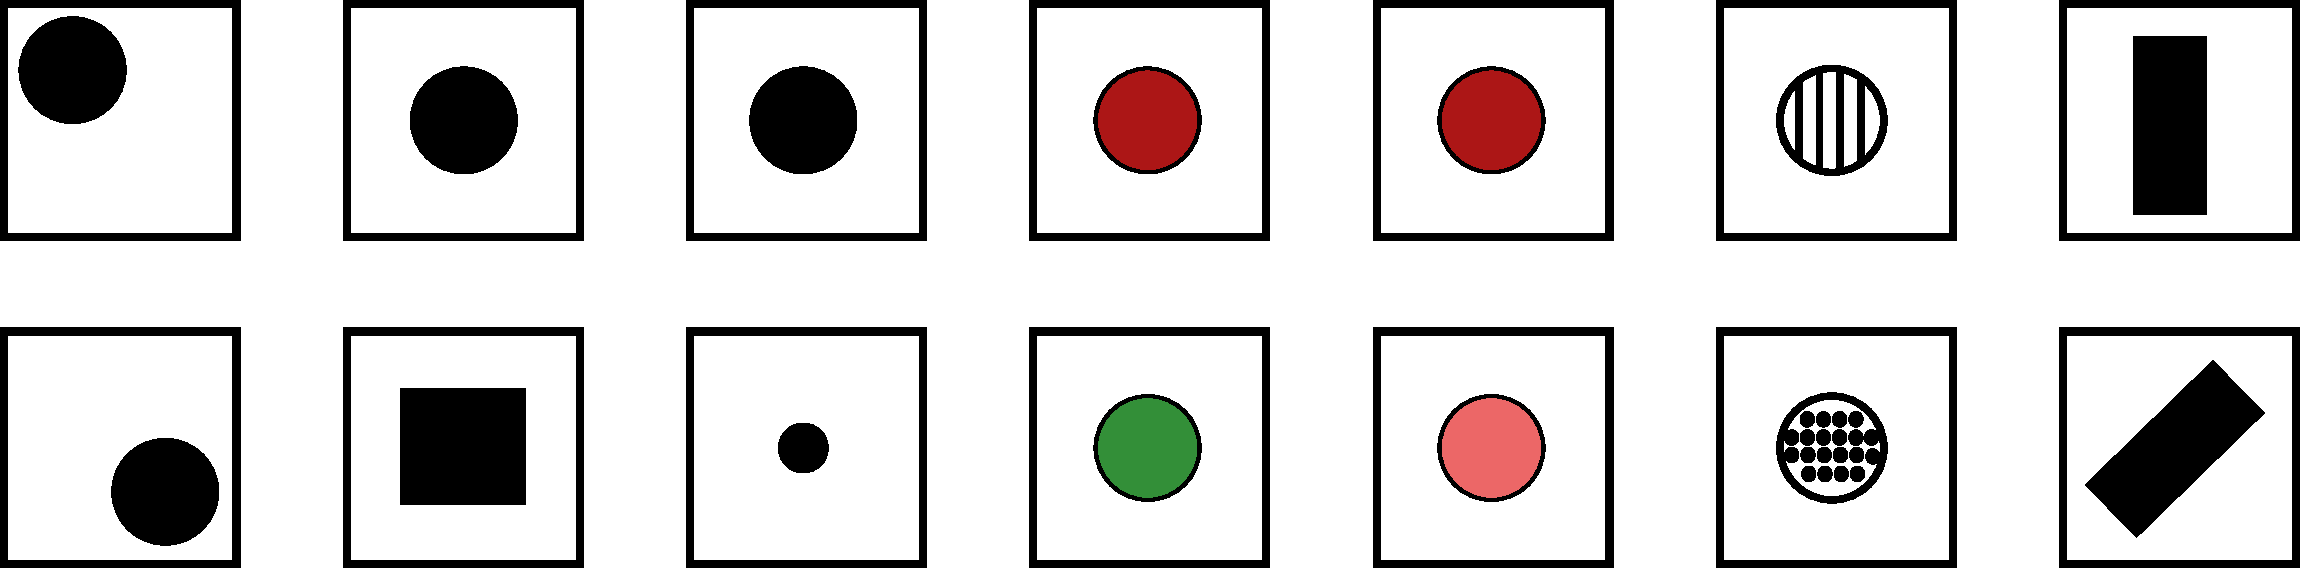
\includegraphics[width=\columnwidth]{Visualization/VisualVariables.pdf}
\caption{\small Visual variables. From left to right: position, shape, size, hue, value, texture and orientation.}
\label{Fig:VisualVariables} 
\end{figure}

These properties are known as \textbf{visual variables} and are applied to the geometric elements used to visualize geographical information. Those elements can be differentiated using the following visual variables, which are shown in figure \ref{Fig:VisualVariables}: position, shape, size, hue, value, texture and orientation.

The use of \textbf{position} is rather restricted in the case of a map, since the real position of the element to be rendered should be respected. It is seldom used. 

The \textbf{shape} is defined by the perimeter of the object. This variable is mostly used in the case of point data, using a symbol of a given shape located at the exact coordinates of the point to be rendered. It is difficult to apply to linear symbols and in the case of areal symbols it requires altering the shape of the symbol itself.

\textbf{Size} indicates the dimensions of the symbol. In the case of points, it can be applied by changing the size of the symbol itself. In the case of lines, changing their thicknesses is the most usual way of applying this visual variable on them. It is not used in areal symbols, except in the case of using a texture fill, in which the size variable is applied to the texture and not to the symbol itself.

Size \textbf{alters how other visual variables are perceived}, especially in the case of small sizes.

\textbf{Texture} refers to the pattern used to fill the body of the symbol. It can be applied to lines, using dash patterns, but it is mostly applied to areal symbols.

Color is the most important of all visual variables. Two of its components can be used as individual visual variables themselves: hue and value.

\textbf{Hue} is what we usually call color. That is, the name of the color (blue, red, green, etc.)

Hue \textbf{can be altered by the hue of surrounding elements}, especially in small symbols. Although human perception has a great sensitivity, it might be difficult to identify in small symbols, and it can be wrongly identified if the symbol has other larger ones with different hues in its surroundings.

\textbf{Value} defines the darkness of the color. For instance, light blue and dark blue have the same hue, but they have different value.

Differentiating two symbols by their value can be difficult depending on the type of symbol. It is easier in the case of areal symbols, while in the case of linear and point symbols it depends on their size. Smaller sizes make it more difficult to compare values and to extract the information that the visual variable is trying to convey.

\textbf{Orientation} is applied to point symbols, unless they have some sort of symetry that makes it difficult to identify the orientation of the symbol. For areal symbols, it is applied to their texture. It's not applied in the case of linear symbols.

\subsection{Properties of visual variables}

Visual variables can have four basic properties.

\begin{itemize}
	\item \textbf{Associative}. A visual variable is said to be associative if, when applied, doesnt change the visibility of an element. That is, it's not possible to give more importance to an element using that visual variable. 
	\item \textbf{Selective}. A visual variable is said to be selective if, when applied, generates different categories of symbols.
	\item \textbf{Ordered}. A visual variable is said to be selective if it can be used to represent a given ordering.
	\item \textbf{quantitative}. When, apart from being ordered, it can be used to express ratios.
\end{itemize}

In the above list, variables are ordered according to the so-called \textbf{levels of organization}. The associative property is at the lower level, while the quantitative one is at the highest. The level of organization of visual variables is relevant when combining them, as we will see later. Also, the level of organization of a variable defines the type of information that the variable can transmit.

Figure \ref{Fig:PropertiesVisualVariables} shows different renderings of a set of point symbols, explaining in each case, one single visual variable.

\begin{figure}[!hbt]
\centering
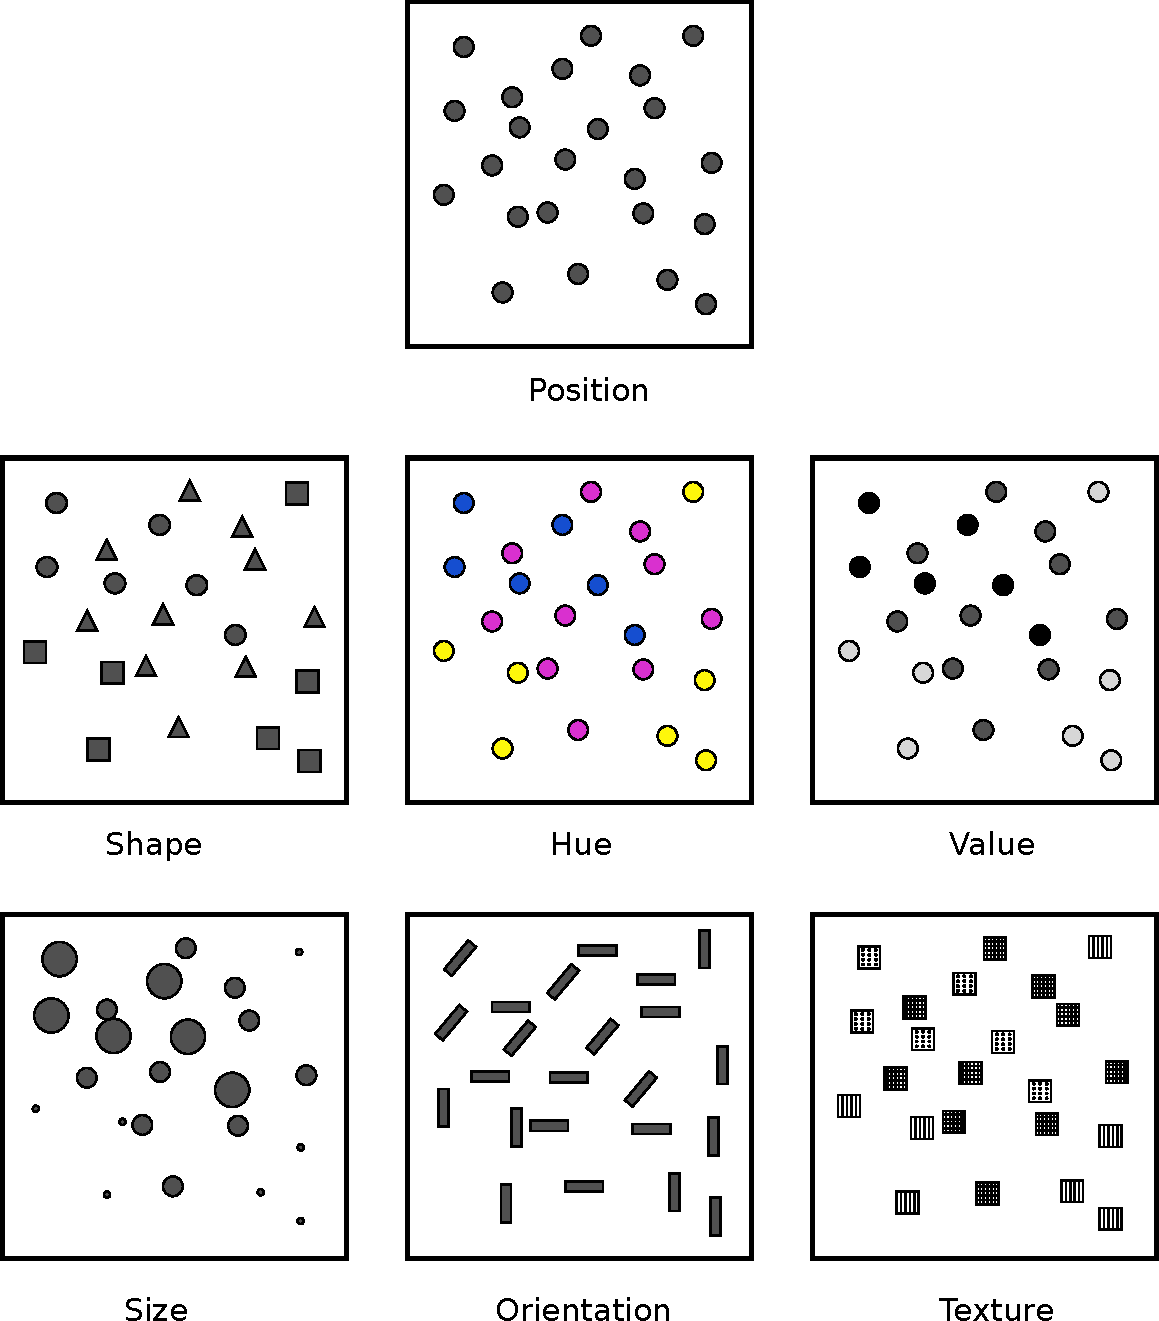
\includegraphics[width=\columnwidth]{Visualization/PropertiesVisualVariables.pdf}
\caption{\small Visualization of a set of point symbols using a single visual variable in each case.}
\label{Fig:PropertiesVisualVariables} 
\end{figure}

Starting with the associative property, we see that, except for size and value, all other visual variables do not do not emphasize one element over the others. In other words, one element is not seen as more important than the rest of them when the visual variable is texture, color, shape or position.

With size, however, it is clear that a larger one gives symbols a more prominent role. In the same way, a darker value attracts the attention of the observer much more than a color with a lighter value.

Regarding the selective property, we can say that a variable has a selective quality if, at a quick glance, we can easily identify the elements that belong to a given group which is defined by a visual variable. The clearest example of this is hue. We can quickly separate from a set of symbols those that are red or yellow. All visual variables, excepting shape, have this property, although it might not be so as in the case of hue. Shape does not make elements form groups spontaneously.

The ordered property is found in those visual variables that we can use to define an ordering. Only position, texture, size and value are ordering properties.  For instance, in the image corresponding to the visual variable hue, we cannot say which element we would place at the beginning or end of a scale defined by hue itself. With value, however, we can, since that scale would range between the lighter tones to the darker ones, and we can visually differentiate and sort them.

Finally, the quantitative property is found in those visual variables that can be used to visually estimate quantities and ratios. Only position and size have it. For instance, we can see that the big circles in the image corresponding to the size visual variable are more or less twice the size of the smaller ones.

Table \ref{Table:PropertiesVisualVariables} contains a summary of all these ideas.

\begin{table}[!hbt]
\small
\centering  \label{Table:PropertiesVisualVariables}
\begin{tabular}{p{3.6cm}ccccccc}  
 & \rotatebox{90}{\textbf{Position}} & \rotatebox{90}{\textbf{Size}} & \rotatebox{90}{\textbf{Shape}} & \rotatebox{90}{\textbf{Value}} & \rotatebox{90}{\textbf{Hue}} & \rotatebox{90}{\textbf{Texture}} & \rotatebox{90}{\textbf{Orientation}} \\ \midrule   
\textbf{Associative}& $\diamondsuit$ & - & $\diamondsuit$ & - & $\diamondsuit$ & $\diamondsuit$ & $\diamondsuit$ \\
\textbf{Selective}& $\diamondsuit$ & $\diamondsuit$ & - & $\diamondsuit$ & $\diamondsuit$ & $\diamondsuit$ & $\diamondsuit$ \\
\textbf{Ordered}&$\diamondsuit$ & $\diamondsuit$ & - & $\diamondsuit$ & - & - & - \\
\textbf{Quantitative}& $\diamondsuit$ & $\diamondsuit$ & - & - & - & - & -  \\
\bottomrule \end{tabular}
\caption{\small Properties of visual variables.}
\end{table}

Visual variables can be combined (for instance, representing objects with different size and hue). The properties of all the visual variables that are used must be considered, and if a given property is needed for the information that we want to convey, all those visual variables should have it.

\subsection{The perception of visual variables}

The perception of visual variables \textbf{might be altered by the environment}. It is important to study this from two points of view: \textbf{perceptual constancy} (how much we can modify visual elements and their surroundings before they fail to to convey the same information and can be misidentified) and \textbf{perceptive aids} (how we can help visual elements to be perceived exactly in the way that we want).

Perceptual constancy defines how objects are \textbf{perceived in the same way regardless of the changes in the environment}. For instance, if an object is round, such as a wheel, it will have a round shape when we look at it from a perpendicular direction. If we now look at it from a different angle, we will see an ellipse instead of a circle. However, we will read it as round and will still identify its shape correctly. That is an example of the perceptual constancy of the shape.

Not all visual variables have such a perceptual constancy. When the perception of an element changes even if the object itself does not, a \textbf{perceptual contrast} is said to exist. Perceptual contrast might cause a visual element to be wrongly perceived and the information that it transmits to be misinterpreted.

The following are some of the main ideas about perceptual contrasts to take into account when creating a map:

\begin{itemize}
	\item Size is the visual variable that is more affected by perceptual contrasts. The apparent size of an object might change if it is surrounded by other elements of a different size. This is particularly relevant when using point symbols in a map.	
	\item Values is also altered when other elements with a different value appear nearby, specially if there are a large number of them.
	\item Hue is altered by the presence of other hues. In a map, we should consider how the background color might affect the foreground symbols. 
	\item Complementary hues, when put together, might cause a vibration sensation in the border between them.
\end{itemize}

Regarding perception aids, the most important factor when creating a map is the \textbf{correct separation between the figure (the foreground objects) and the background}. The properties of the visual variables must be used to create different levels in the visualization, assigning more relevance to some elements in order to focus the attention on the information that they transmit.

To make certain layers (the most relevant ones for the purpose of the map) more visible, a \textbf{correct hierarchy} must be established with the help of visual variables. This hierarchy will add depth to the information displayed in the map, and some elements will be perceived as being more important than others. Layer ordering already defines a structure and a hierarchy, but that is not enough in most cases and visual variables should be used to reinforce it.

Figure \ref{Fig:HierarchyMap} shows why a correct hierarchy is needed to create a good map.

\begin{figure}[!hbt]
\centering
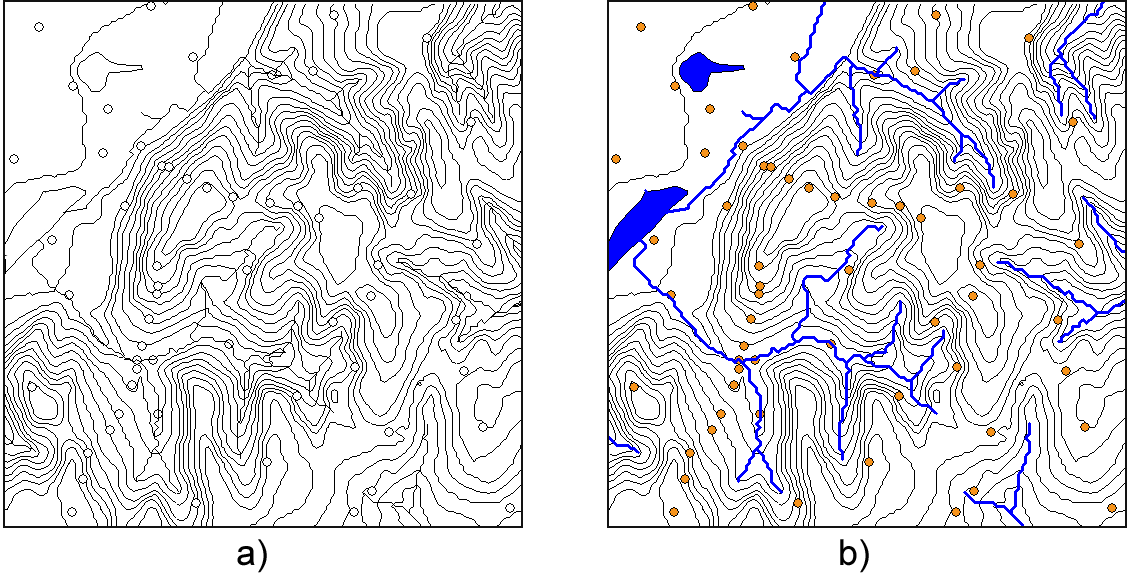
\includegraphics[width=\columnwidth]{Visualization/HierarchyMap.png}
\caption{\small Comparison between a map without hierarchy (a) and a map with a correct hierarchy (b).}
\label{Fig:HierarchyMap} 
\end{figure}


\section{Maps and cartographic communication}

Maps are a method of communication that uses a language with a particular purpose: \textbf{describing spatial relations}. A map is, therefore, a symbolic abstraction of a real-word phenomenon, which implies that it has some degree of simplification and generalization.

The visual language that we have just seen becomes a cartographic language when it is adapted to the particular case of creating maps and knowing its rules is needed to create cartography that is later useful for the map user. All these ideas related to map production form what is known as \textbf{cartographic design}.

Cartographic design involves making decisions (in this case, by the GIS user who takes the role of the cartographer). These decisions must be guided by the \textbf{purpose of the map} and the \textbf{target audience} and depending on these factors, the cartographer must decide \textbf{the projection} (which doesn not always have to be the original one of the data), the \textbf{scale} (depending on the level of detail and taking into account the limitations of the data), the \textbf{type of map} (we will see more about this later in this chapter), or the \textbf{symbols} to use, among other things.

There are two main types of cartography: \textbf{base cartography} (also called \textbf{fundamental} or \textbf{topographic}) and \textbf{thematic cartography}.

Historically, base cartography represents the classic maps that have been created by cartographers. This type of map serves the purpose of precisely describing \emph{what} is on the surface of the Earth.

Thematic cartography focuses on \textbf{displaying information about a given phenomenon} (a given geographical variable), which can be of any type: physical, social, political, cultural, etc. We exclude from this list those phenomena that are purely topographic, which are the subject matter of base cartography.

We can also say that base cartography represents \textbf{physical elements} (a stream, a coast line, a road, a valley, etc.), while thematic cartography focuses on \textbf{representing values and attributes}.

Thematic cartography uses base cartography (usually included in thematic maps) to help the map user to understand the spatial behavior of the variable being represented, and also to provide a geographical context for it.


\subsection{Types of information and their visualization}

We already know that the thematic component of geographical information can be numeric or alphanumeric and that numeric variables can be nominal, ordinal, intervals, or ratios. Selecting a correct symbology according to the type of information that we are working with is key to producing an effective map. In particular, we must use a visual variable that has the correct properties (levels of organization) for the variable that we want to visualize.

For instance, the associative property and the selective property are of interest just for qualitative information, while size is the only visual variable that we can use that has the quantitative property and therefore, the only one that should be used to represent ratios.

The following are some of the more important ideas about this, referred to the aforementioned types of information.


\begin{itemize}
	
	\item \textbf{Nominal}. Nominal information is correctly represented using the visual variable shape. This information shows \emph{what} is found in the different locations of a map, and not \emph{how much} is found, and it is more related to base cartography than to thematic cartography. Using different symbols for point elements and line elements is a common and very effective solution. For the case of areal symbols, hue and texture are the most common solutions.

	Alphanumeric information has similar properties, and the same ideas apply to it.
	
	\item \textbf{Ordinal}. Since values of the variable define an order, a visual variable with the ordered property is needed to correctly visualize this type of information
	
	\item \textbf{Interval and ratio}. Visual variables with the ordered property can be used in this case. However, size is a better choice, as it is the only one which has the quantitative property.

	Values are normally grouped into classes so the same value of the visual variable (same size of the symbols or same color value, for instance) is used for different values of the variable that we are visualizing. There are different strategies for this, which try to maximize the information that the map transmits. The most commons ones are \textbf{equal intervals, intervals using percentiles} or \textbf{natural intervals} (intervals that try to minimize the variance within each class).

	Using one or another of these methods can have a noticeable effect in the visualization, as is shown in figure  \ref{Fig:IntervalClasses}.

	\begin{figure}[!hbt]
	\centering
	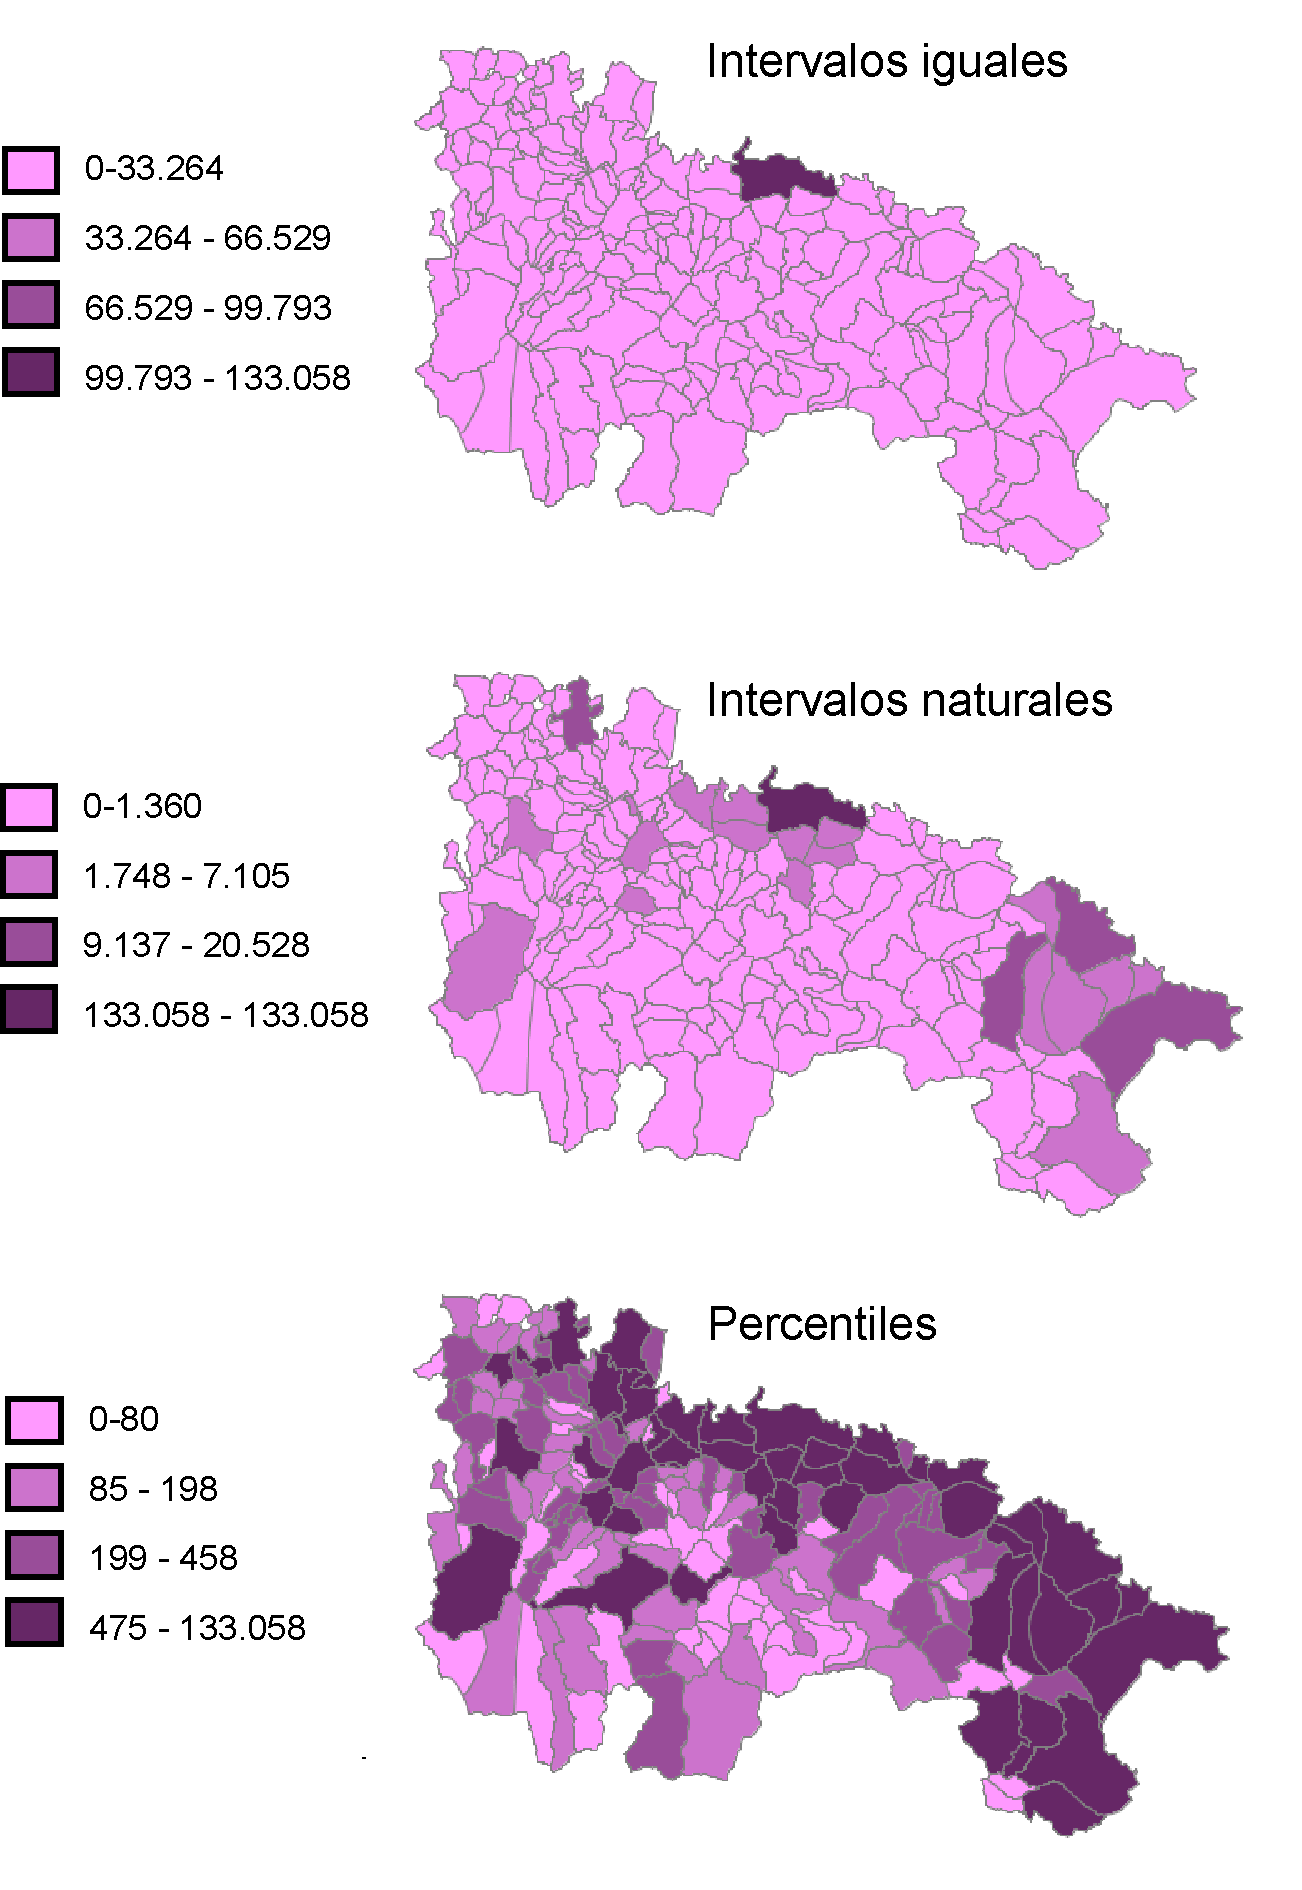
\includegraphics[width=.7\columnwidth]{Visualization/IntervalClasses.pdf}
	\caption{\small Comparison between different methods of defining intervals.}
	\label{Fig:IntervalClasses} 
	\end{figure}


\end{itemize}


It is important to remark that, although levels of organization indicate increasing potential (that is, with a variable such as size or value we can convey all the information that can be conveyed with hue, since they have properties with a higher level), \textbf{it is not always better to use visual variables with a higher level of organization}, and it is not true that they will always be better than those with a lower one. For instance, using the visual variable value for a map with qualitative information (like using a ramp of different tones of blue for a map with soil type information) might not be a good idea, because it has the ordered property, and that might cause the map user to think that there is some hierarchy (that some soil types are ``better'' than others), which is false.


\subsection{Map elements. Map composition}

A map is not just the part that represents the geographical information, but a set of multiple elements, for example, the one that contains the geographical information itself.

A \textbf{correct layout of the map elements} is as important as a correct symbology, since these, like symbology itself, are designed to help the map user to better interpret the information that it contains.

The following are the main elements that can be used to compose a map (Figure \ref{Fig:MapElements}):

\begin{figure}[!hbt]
\centering
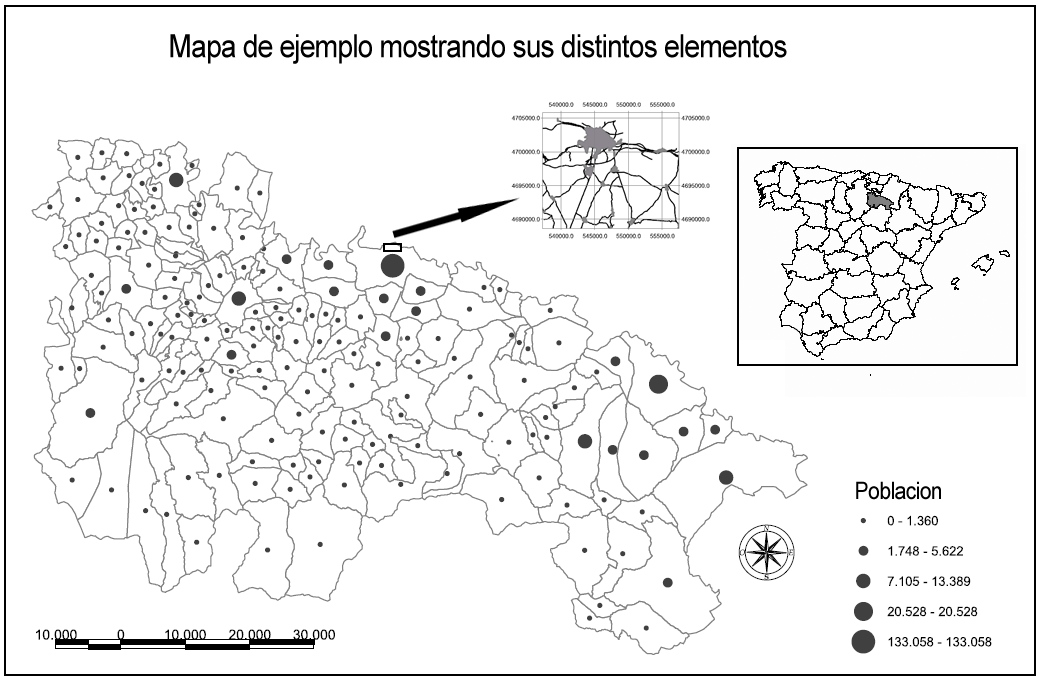
\includegraphics[width=\columnwidth]{Visualization/MapElements.png}
\caption{\small Map with its most common elements.}
\label{Fig:MapElements} 
\end{figure}

\begin{itemize}
\item \textbf{Name or title}. Needed to know what information is contained in the map.
	\item \textbf{Author}. Creator the map.
	\item \textbf{Additional information about the map}. For instance, the coordinate reference system used or its creation data, among others.
	\item \textbf{Data frame}. The frame which contains the rendered geographical information. It is the central element and will use most of the space of the map. 
	\item \textbf{Graticule}. On top of the data frame, it locates the content of the map on the Earth and provides a geographical reference. It serves the same purpose as the scale, helping to estimate distances. It is usually added at all scales, but it is more relevant in the case of small scales.
	\item \textbf{Legend}. When designing a map, we should try to use a symbology that is as expressive as possible. However, sometimes it is not possible to include all the information with just the symbology itself and a legend is required. The legend has to be clear and easy to interpret as well. A legend that is too large or difficult to understand is probably telling us that the symbology that we have selected can be improved.
	
	The legend and the data frame form a single unit and should be together (legend inside the data frame), not separated in different frames or with boundaries between them, unless the data frame uses all the space of the map and it is not possible to visually separate both elements clearly.
	

	\item \textbf{North arrow}. Although by convention maps have a south-north orientation (north is at the top of the map), it does not always have to be that way. An arrow pointing north or a compass rose will help to clarify the map orientation.
	\item \textbf{Scale}. Map scale should be displayed both numerically and graphically (scale bar).
	\item \textbf{Locator map}. Allows the user to locate the map in a larger geographical context. It is especially relevant in the case of map series, to show the relation between the current map and the rest of them, acting as an index map.
	\item \textbf{Detail maps}. Used when there is an area that we can show with a greater level of detail. The area that it corresponds to should be indicated as well in the main map. 
\end{itemize}

It is also important that the map \textbf{emphasizes its purpose}, giving more importance to those element that serve it better.

\section{Types of thematic maps}

There are many different ways of visualizing a given variable in a map. Several of them can be combined in a single map, especially if it includes more than one variable. In this case, the combination should strive to obtain the maximum possible clarity for all of them so the rendering of a variable does not overshadow the remaining ones.

In this section, we will describe the following types of thematic maps: proportional symbol maps, point density maps, isoline maps and choropleth maps.


\subsection{Proportional symbol maps}

A proportional symbol map represents \textbf{quantitative variables} using symbols whose size \textbf{is proportional to the value} of the variable. That is, it uses the visual variable size (the only one with the quantitative property), to transmit the value of the variable being represented. If the symbol used is linear (such as a bar), its length is used to scale the values to render. If it is areal, area is used. That means that, in case of using circles, a value three times larger than a reference one will not be rendered with a circle with a radius three times longer, but with a circle with an area three times the area of the reference circle.

Symbol scaling can be done in a continuous way, but it is usually more convenient to use a discrete approach, grouping values in classes and assigning a single size for all values in each class, usually the size that corresponds to the center value of the class. 

To avoid problems when perceiving the size of each symbol, it is important to show in the legend the relation between the different sizes and their corresponding values, as can be seen in figure \ref{Fig:LegendProportionalSymbols}

\begin{figure}[!hbt]
\centering
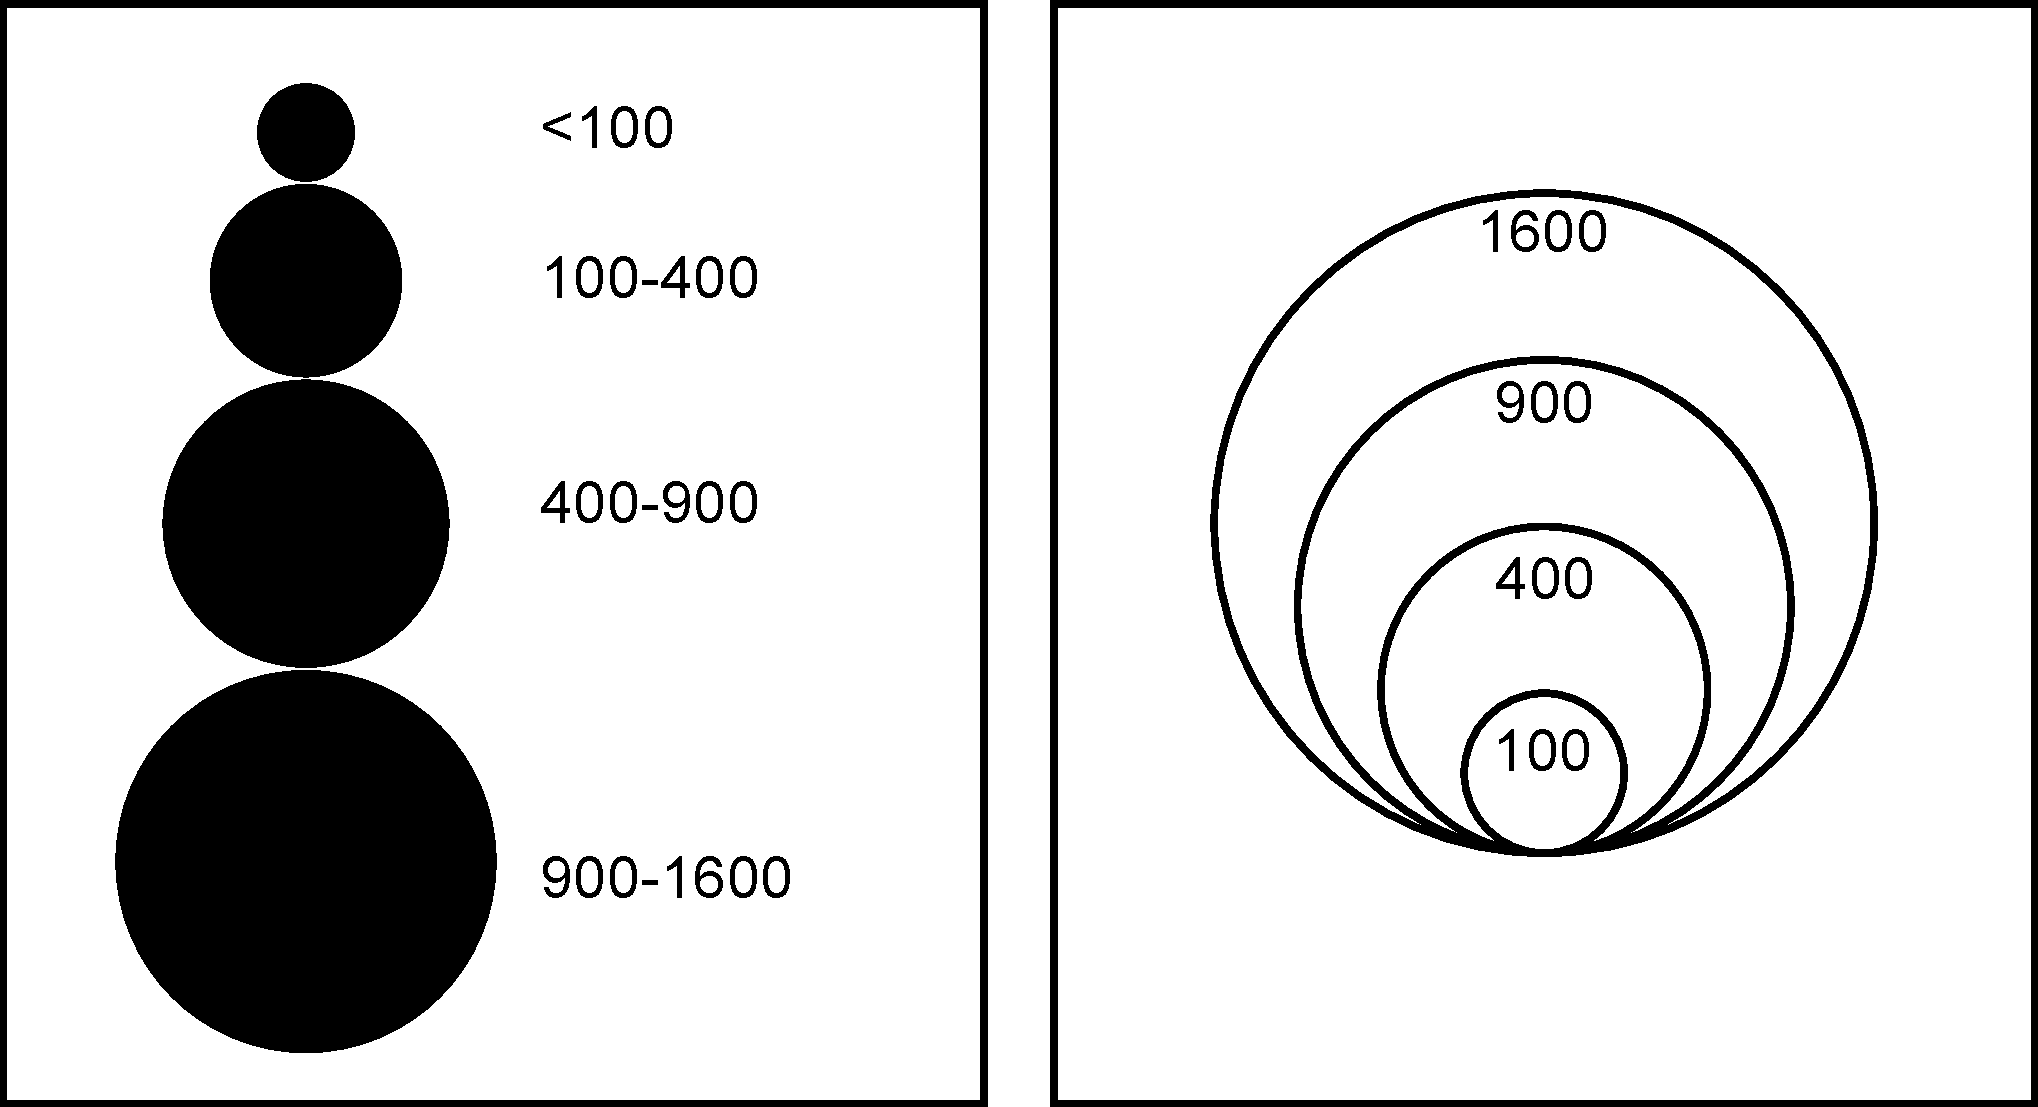
\includegraphics[width=.65\columnwidth]{Visualization/LegendProportionalSymbols.pdf}
\caption{\small Two types of legend for proportional symbols maps.}
\label{Fig:LegendProportionalSymbols} 
\end{figure}


\subsection{Point density maps}

Point density maps are particularly suitable for countable variables such as population or crop yield. These quantities are represented using \textbf{repeated points}, whose number is proportional to the quantity itself. Each point represents a unitary value, and all the points within an area add up to the total value of the variable in it. All points have the same size and shape, unlike what we saw in the case of proportional symbols.

When creating a point density map, three parameters have to be defined: the \textbf{value of each point} (that is, how many units of the variable the point represents), its \textbf{size} and its \textbf{position}.

The value of each point should be defined \textbf{based on the range of values} covered by the variable, so points in the resulting map are not too scarce or too numerous. This value will be included in the legend, usually in text form, writing, for instance, that ``a point represents 1000 inhabitants''.

Size must guarantee that points are visible and at the same time they do not take too much space in the map. The \textbf{optimal size is linked to the selected value of each point}, and both parameters should be considered together, so as to find the best combination of them. 

The position of the points is of great importance, as it should not convey wrong information or cause the user to misinterpret its meaning. If we do not have any additional information, points should be regularly distributed, covering the whole area that correspond to the variable value. If, on the other hand, we have more information about the distribution of the variable, we should use it to give the points a more realistic position. For instance, if we are creating a density map with population values for regions, there should be more points in the surroundings of the cities within the region, since there are more inhabitants in those areas.

Another thing to consider is the meaning of the variable and whether or not the phenomenon that it represent can appear at a given point. For instance, if the variable that we are representing is the number of water birds know to nest in each region, it will be wrong to place the density points in forest areas or city ones, since it might be inferred that birds are found there, which is not true.

Image \ref{Fig:MapPoints} shows an example of a point density map.


\begin{figure}[!hbt]
\centering
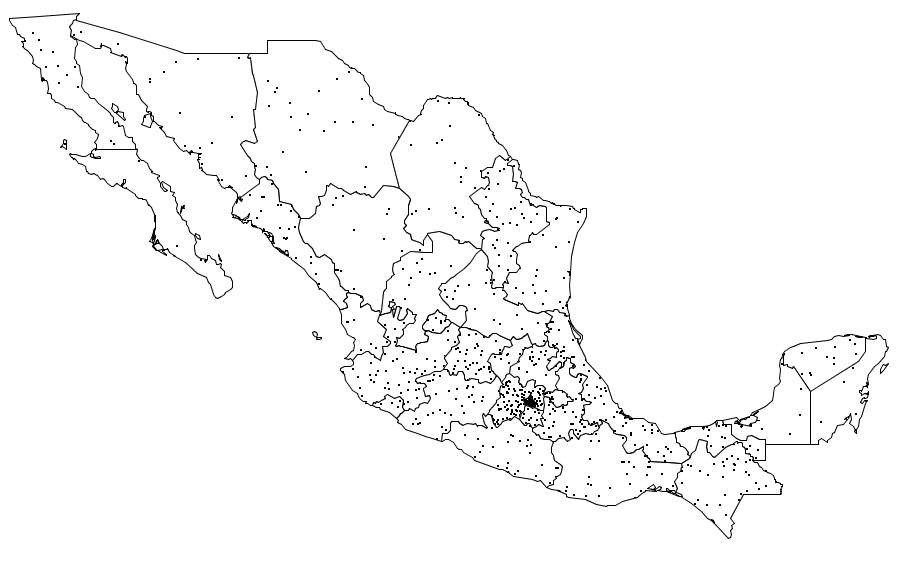
\includegraphics[width=.8\columnwidth]{Visualization/MapPoints.png}
\caption{\small Point density map.}
\label{Fig:MapPoints} 
\end{figure}


\subsection{Isoline map}

Isoline map are commonly used to represent \textbf{continuous variables}. Containing only lines, they mix well with other types of maps without being  obtrusive.

An isoline map is formed by a set of lines, each of them connecting points that have the same value of the variable being represented. These lines cannot cross with each other, since a point cannot have two values at the same time. The most common use of isolines are contour lines in topographic maps, which represent points with the same elevation.

Isolines are defined by their \textbf{equidistance}, which indicate the difference between the values represented by any two contiguous isolines. A lower equidistance means more isolines and a denser map.

Size is the only visual variable used with isolines. It is used to highlight those that represent a value that is multiple of a given number, to make the map easier to read. These lines are know as \textbf{index lines}.


\begin{figure}[!hbt]
\centering
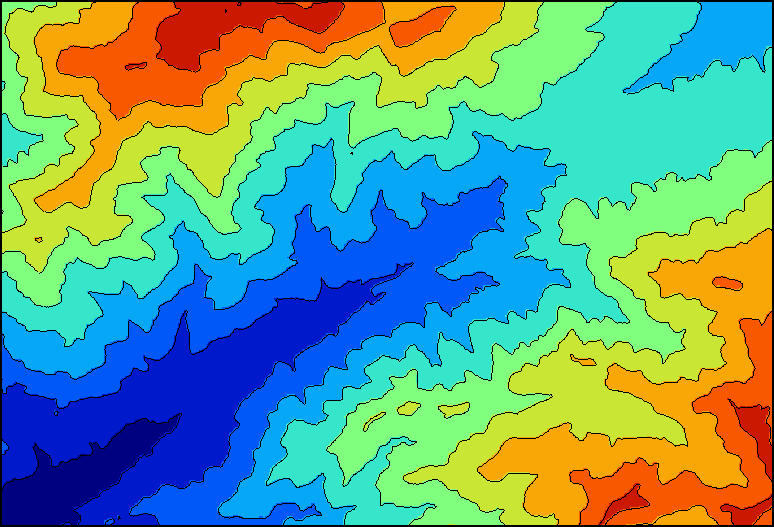
\includegraphics[width=.8\columnwidth]{Visualization/Isolines.png}
\caption{\small Map with isolines and hypsometric tints.}
\label{Fig:Isolines} 
\end{figure}


Lines are labeled with their value over the line itself, usually only on the index lines (the value of other lines between the index ones can be easily figured out knowing the equidistance).

A particular case of isolines are the so called \textbf{hypsometric tints}. Apart from drawing the lines themselves, the areas between them are colored, each with a different color (usually using a graduated scheme).

Figure \ref{Fig:Isolines} shows an example of this.

\subsection{Choropleth maps}

Choropleth maps are a very common type of map in GIS. For instance, maps in figure \ref{Fig:IntervalClasses} were all choropleth maps.

In a choropleth map, there is a set of areas, each of them representing a single value of a variable. This value applies to the whole area, and is normally represented using hue applied to the areal symbol.

Choropleth maps have some  important limitations. One of them is the \textbf{sharp change in the boundaries between areas}, which might be interpreted as a abrupt change in the variable value in that boundary. This could hide the continuity of the variable distribution, in case it exists. Another problem is the \textbf{homogeneity within each area}, which might lead to thinking that the variable has a uniform distribution, even if that is false.

In many cases, and in order to correctly transmit the information contained in the variable, its values have to be \textbf{normalized using the area of each region}.


\section{Visualization in a GIS}

Now that we know the basic ideas about visualization and how they are applied to maps, it is time to see how these are used in the context of a GIS. Two ideas are particularly relevant in this contexts: the fact that we work with \textbf{multiple layers} to be represented together, and the particularities of \textbf{on-screen rendering and the interactivity it offers}.

\subsection{Combining multiple layers}

In most cases, visualizing a layer alone by itself is not the best way of visualizing the information it contains. In a map, we normally find several types of information, and that is not just for the sake of space, but because it helps the map user to understand and interpret the main information. For instance, contour lines help to understand the meaning of rivers and lakes, providing a valuable context.

When combining layers, we should try to create a synergy between them, so they complement each other. This is mostly done by \textbf{correctly ordering the layers} and using \textbf{a symbology for each of them that does not interfere with the others}.

When two layers have information for the same location, only the information of the layer on top will be seen. Layer ordering should maximize the information that is seen in the map, and prioritize the most important layers over those that contains secondary information.

We know that raster layers fill the space and contain values in all of their cells (pixels in the case of an image). For this reason, they will cover whatever is underneath, and is not a good idea to place them at the top of the rendering order. Instead, they should be considered as \textbf{base layers on top of which the remaining layers are placed}.

With a similar reasoning, we can define the best way to order vector layers, placing polygon ones first, then line ones, and then point ones at the top of the rendering order.

Sometimes, the rendering order \textbf{might be imposed by the meaning of layers}. For instance, if we are creating a map with a layer containing streams and another one containing roads, this last one should go on top of the first one, since roads usually pass over streams and not the other way round.

A common functionality that most GIS have is the use of \textbf{transparency} for layer. It can be applied to both raster and vector layers. Figure \ref{Fig:Transparency} was created using this technique. The polygon that defines the boundary of the watershed has a semi-transparent fill, which allows to see the shaded relief layer underneath. The result is a map in which the hydrogical meaning of the watershed is much clearer and easy to understand.

\begin{figure}[!hbt]
\centering
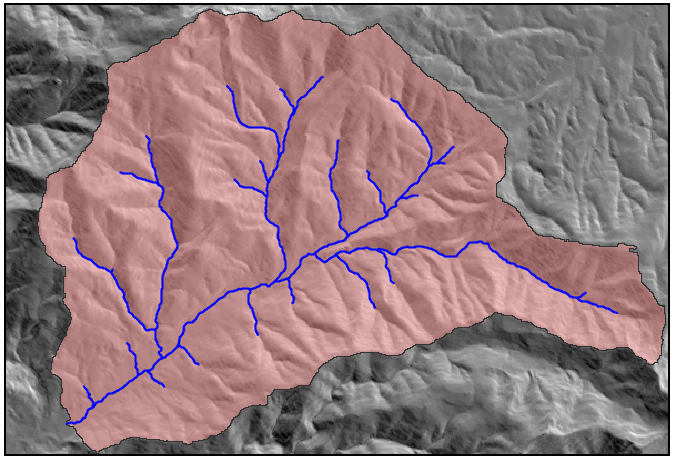
\includegraphics[width=.7\columnwidth]{Visualization/Transparency.png}
\caption{\small Combination of two layers using transparency.}
\label{Fig:Transparency} 
\end{figure}

In the case of raster layers, transparency can be applied partially, just rendering those cells that are within a given range of values.

If a variable is divided in many \textbf{separate layers} (horizontal division), the \textbf{same symbology} must be applied to all of them, in order to have a coherent map.


\subsection{Particularities of on-screen rendering}

Apart from the ideas that are applied to printed maps, additional ones must be taken into account when the visualization takes place instead on a computer screen. A printed map should not be designed in the same way as a map that is meant to be rendered on the screen.

The main elements to consider are the \textbf{low resolution of the screen} when compared to a printing device, and the \textbf{interactivity} of the visualization itself.

When creating a printed map, resolution is not a problem, since printing devices offer a level of detail that goes beyond what the cartographer might need. However, screen resolution is much lower and certain elements might not be rendered with enough clarity. Although these elements can be used in printed maps, they should be replaced for on-screen maps. Among these problematic element we find \textbf{fonts with ornaments} such as shades, \textbf{fonts with serifs} (small lines attached to the end of the stroke to increase readability) or \textbf{texture fills of small size}.

Regarding interactivity, we must take into account that, unlike a printed map, an on-screen map is not a static element, but a dynamic one. That does not mean that the map changes by itself, but instead that the user can alter it using the tools that we have already seen (zoom, pan, etc.)

Since the scale can be changed by the user, that might cause problem with certain elements such as symbols and text labels. If all elements are scaled proportionally, reducing the scale will make the labels too small and impossible to read. On the other hand, if the scale is increased, labels might be too large, as can be seen in figure \ref{Fig:ProblemsChangeScale}. 


\begin{figure}[!hbt]
\centering
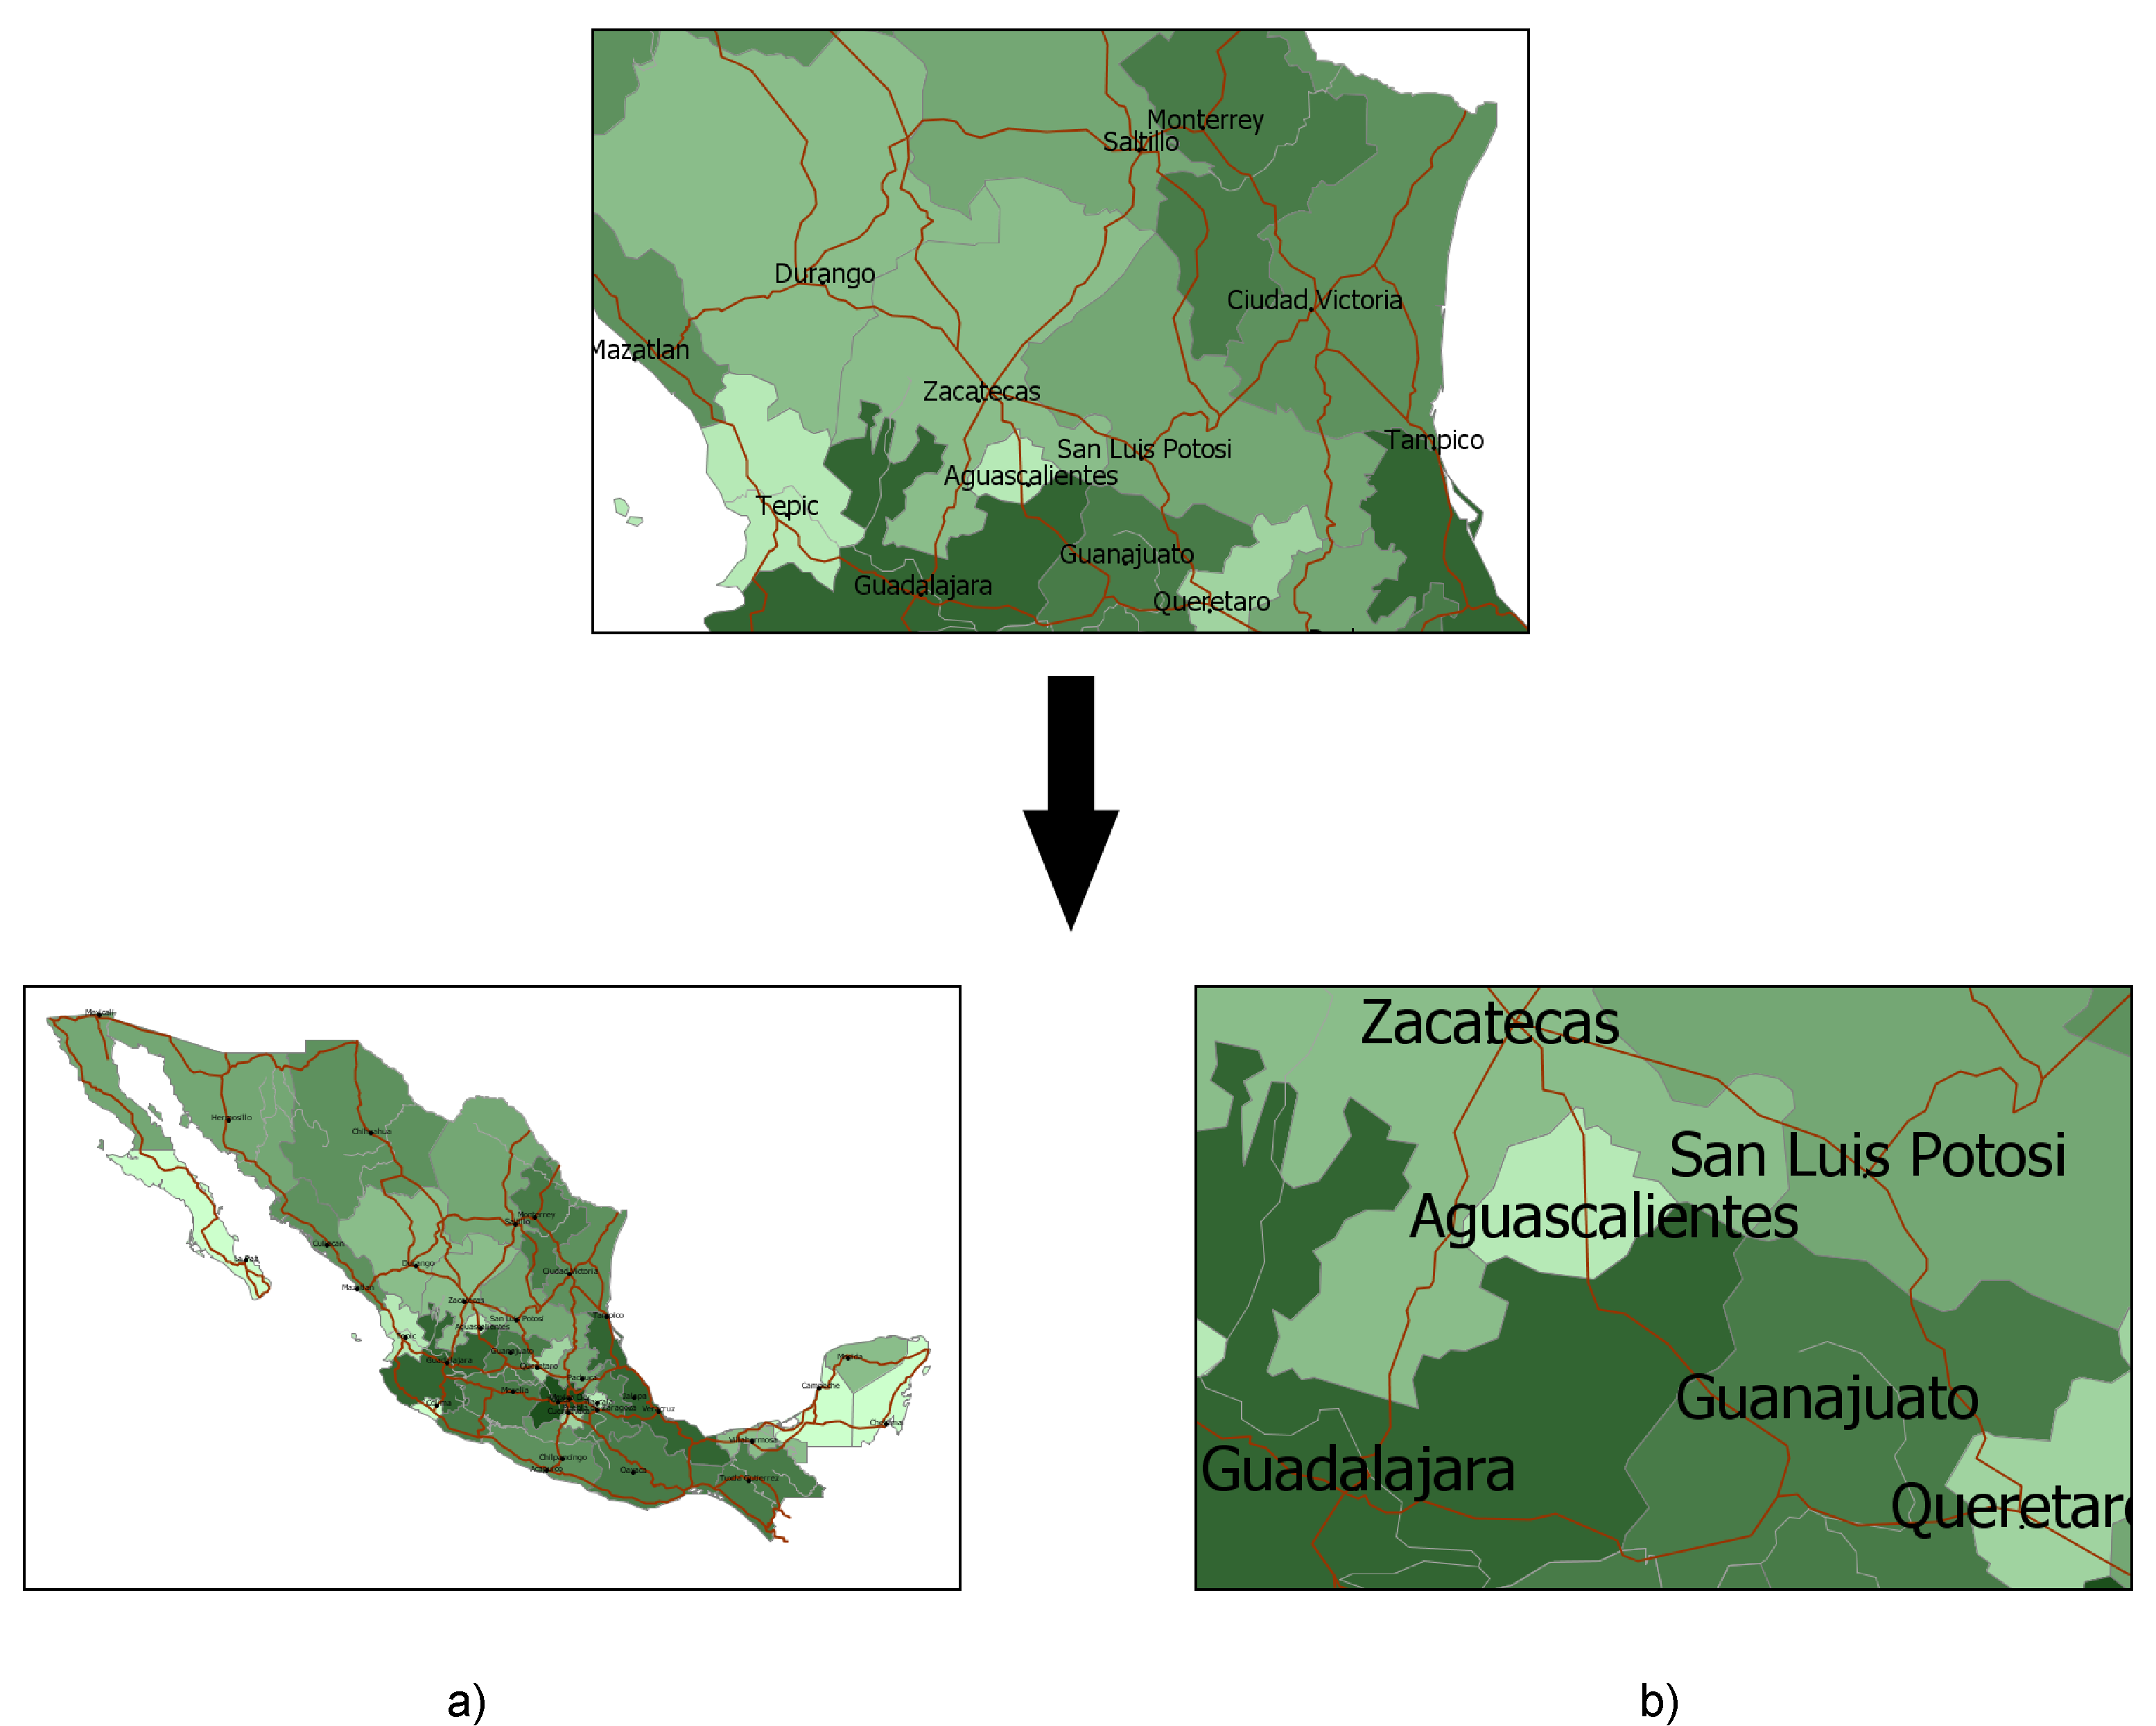
\includegraphics[width=\columnwidth]{Visualization/ProblemsChangeScale.pdf}
\caption{\small  A scale change modifes the size of symbols and text labels, and it can make them too small (a) or too large (b).}
\label{Fig:ProblemsChangeScale} 
\end{figure}

A solution to that is to use an \textbf{absolute size} for those elements, so they always have the same size regardless of the scale. With lower scales, however, that might result in maps that are saturated, as can be seen in figure \ref{Fig:SaturatedMap}.

\begin{figure}[!hbt]
\centering
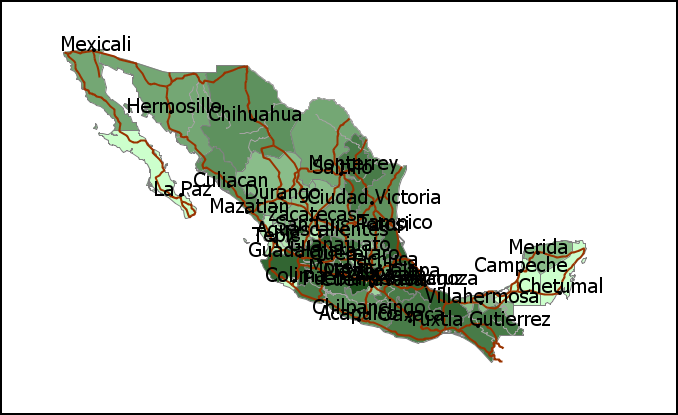
\includegraphics[width=.9\columnwidth]{Visualization/SaturatedMap.png}
\caption{\small Saturated map caused by rendering elements at a fixed size at a low scale.}
\label{Fig:SaturatedMap} 
\end{figure}

The ability of GIS to render layers at different scales can also cause \textbf{performance issues}. At low scales, the number of elements to be rendered can be too large, and painting them on the screen might take too much time. To avoid these problems, a \textbf{multiscalar approach} can be adopted, in which, depending on the scale, different layers and elements are rendered. For the same information, different versions with different levels of detail can be used, each of them being used only at a given scale range.

\pagestyle{empty}